\chapter{Balança}
%\setcounter{section}{0}
%%%%%%%%%%%%%%%%%%%%%%%%%%%%%%%%%%%%%%%%%%%%%%%%%%%%%%%%%%%%%%%%
As balanças foram criadas por necessidade, quando o desenvolvimento de comercio durante a antiguidade os produtos que não recorriam a contagem por unidades, tais como objetos irregulares por exemplo o ouro devia ser valorizado, a forma de medir sua massas tornou-se numa variável de medição para troca de bens.\\
\\
A relíquia mais antiga de uma balança de medir massa foi descoberto na vila de \textit{Indus River}, perto do conhecido por hoje de Pakistão, e estima-se ser por volta de 2000 B.C.\\
Estas primeiras balanças eram alavancas em equilíbrio, onde nos extremos eram colocados cestos e se colocava os pesos, este estava centrado no seu centro de massa, assim se os pesos nos dois cestos serem iguais fica em equilíbrio (horizontal), era um sistema de comparar com pesos fixos estabelecidos como norma (\textit{contra-pesos}).
\\
\begin{minipage}[!b]{0.45\linewidth}
	\begin{figure}[H]
		\centering
		\includegraphics[height=7cm]{./image/PESTA/general/balanca_1.jpg}
		\caption{Balança medieval}
		\label{balanca_1}
	\end{figure}
\end{minipage}
\hspace{2.2cm}
\begin{minipage}[!b]{0.45\linewidth}
	\begin{figure}[H]
		\centering
		\includegraphics[height=7cm]{./image/PESTA/general/balanca_4.jpg}
		\caption{Balança moderna}
		\label{balanca_4}
	\end{figure}
\end{minipage}
\newline
\newline
\newline
Este sistema pode ter grande precisão, mas também pode facilmente ser adulterado.
\\
\\
Os métodos de medir a massa de objetos não conheceu nenhumas melhorias tecnológicas relevantes até a era industrial. Só nos fins do século \textit{XVIII} é que o meio de medir a massa de objetos não dependia de \textbf{contra-pesos}. As balanças por molas foi inventado por \textbf{\textit{Richard Salter}}, um fabricante de balanças por volta dos anos de 1770 na Inglaterra.\\
\begin{minipage}[!b]{\linewidth}
	\begin{figure}[H]
		\captionsetup{justification=raggedright,singlelinecheck=false}
		\flushleft
		\includegraphics[height=7cm]{./image/PESTA/general/Public_Body_Scales_1.jpg}
		\hspace{.8cm}
		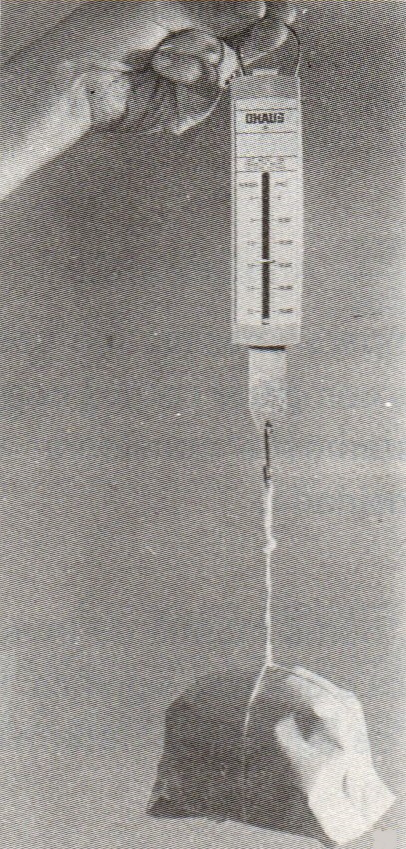
\includegraphics[height=7cm]{./image/PESTA/general/Balanca_Mola_1.jpg}
		\caption{Balança de Mola}
		\label{Balanca_Mola_1}
	\end{figure}
\end{minipage}
\newline
\newline
\newline
A balança por mola, como o nome implica, mede a pressão (ou sua tensão) exercido sobre a mola para determinar a massa do objeto. Este tipo de balanças ainda são muito comum nos dias de hoje por serem bastante económicas de fabricar, mas não tem tanta precisão como as eletrónicas desenvolvidas e aperfeiçoadas durante o século \textit{XX}.
\\
\\
As balanças eletrónicas mais modernas utilizam resistências elétricas em materiais permeáveis e fazer passar uma corrente elétrica na qual é possível detetar a variação de condutividade das resistências em que é proporcional a pressão exercida sobre esse material, podendo dai se deduzir o peso dos objetos que se encontrem na balança.
\\
\\
\\
\section{section}
\subsection{subsection}
\subsection{subsection}
\section{subsection}
